% !TeX spellcheck = da_DK
% Setup document class.
%  This will always be the beamer class, but depending on the use of notes,
%  it can be annotated with the option [notes] or  [notes=only], depending
%  on whether notes should be included, or should be the only thing in
%  the document.
\documentclass[c]{beamer}

% Setup theme.
%\usetheme[
%%% options passed to the outer theme
%    progressstyle=fixedCircCnt,   %either fixedCircCnt, movCircCnt, or corner
%    rotationcw,          % change the rotation direction from counter-clockwise to clockwise
%    shownavsym          % show the navigation symbols
]{AAUsimple}

\usetheme[
%%% options passed to the outer theme
%    hidetitle,           % hide the (short) title in the sidebar
%    hideauthor,          % hide the (short) author in the sidebar
%    hideinstitute,       % hide the (short) institute in the bottom of the sidebar
%    shownavsym,          % show the navigation symbols
%    width=2cm,           % width of the sidebar (default is 2 cm)
    hideothersubsections,% hide all subsections but the subsections in the current section
%    hideallsubsections,  % hide all subsections
    left               % right of left position of sidebar (default is right)
%%% options passed to the color theme
%    lightheaderbg,       % use a light header background
  ]{AAUsidebar}



% Import preamble
%%% Initial things %%%
% Increase number of dimen registers
\usepackage{etex}
% Fix various issues with LaTeX2e
\usepackage{fixltx2e}
% Font package
\usepackage{fourier}
% Import package
\usepackage{import}
\usepackage{shellesc}


%%% Translations and character encodings %%%
% Enable use of several characters, including æ, ø and å
\usepackage[utf8]{inputenc}
% Danish language
\usepackage[danish]{babel}
% Use PostScript fonts instead of bitmap ones. Also does other stuff.
\usepackage[T1]{fontenc}
% Various LaTeX symbols
\usepackage{latexsym}
% Wider selection of colours
\usepackage{xcolor}
\definecolor{aaublue}{gray}{0}
\definecolor{bluekeywords}{gray}{0}
\definecolor{greencomments}{gray}{0.5}
\definecolor{redstrings}{gray}{0.3}
\definecolor{codebg}{HTML}{EFEFEF}
\definecolor{codefg}{HTML}{000000}
\definecolor{part}{HTML}{34495E}
\definecolor{numbers}{HTML}{34495E}
\definecolor{smartdiagram1}{HTML}{1ABC9C}
\definecolor{smartdiagram2}{HTML}{2ECC71}
\definecolor{smartdiagram3}{HTML}{3498db}
\definecolor{smartdiagram4}{HTML}{9b59b6}
\definecolor{smartdiagram5}{HTML}{E74C3C}
\definecolor{smartdiagram6}{HTML}{F1C40F}
\definecolor{smartdiagram7}{HTML}{E67E22}
\definecolor{diagramDark}{HTML}{19B5FE}
\definecolor{diagramLight}{HTML}{6BB9F0}

\definecolor{tableGoodLight}{HTML}{87D37C}
\definecolor{tableGoodDark}{HTML}{26A65B}
\definecolor{tableBadLight}{HTML}{EC644B}
\definecolor{tableBadDark}{HTML}{EF4836}


\definecolor{GoogleGreen}{HTML}{4CAF50}
\definecolor{GoogleRed}{HTML}{F44336}
\definecolor{GooglePurple}{HTML}{9C27B0}
\definecolor{GoogleDeepPurple}{HTML}{673AB7}
\definecolor{GoogleIndigo}{HTML}{3F51B5}
\definecolor{GoogleBlue}{HTML}{2196F3}
\definecolor{GoogleLightBlue}{HTML}{03A9F4}
\definecolor{GoogleCyan}{HTML}{00BCD4}
\definecolor{GoogleTeal}{HTML}{009688}
\definecolor{GoogleLightGreen}{HTML}{8BC34A}
\definecolor{GoogleLime}{HTML}{CDDC39}
\definecolor{GoogleYellow}{HTML}{FFEB3B}
\definecolor{GoogleAmber}{HTML}{FFC107}
\definecolor{GoogleOrange}{HTML}{FF9800}
\definecolor{GoogleDeepOrange}{HTML}{FF5722}
\definecolor{GoogleBrown}{HTML}{795548}
\definecolor{GoogleGrey}{HTML}{9E9E9E}
\definecolor{GoogleBlueGrey}{HTML}{607D8B}

% Improved element justification
\usepackage{ragged2e}
% Font improvements
\usepackage{fix-cm}
% Enables various forms of lines, like double-underlining (\uuline{})
\usepackage{ulem}
% Sets the tolerance for distance between words, determining when to hyphenate.
\pretolerance=2500


%%% Figures and tables (Floats) %%%
% Enable multi-rows and -columns
\usepackage{multirow}
\usepackage{multicol}
% Double, horizontal lines
\usepackage{hhline}
% Enables coloured tables
\usepackage{colortbl}
% Prettier tables
\usepackage{booktabs}


%%% Mathematic formulas %%%
% AMS math
\usepackage{amsmath}
\usepackage{amssymb}
% Extra fonts (for math, I think)
\usepackage{stmaryrd}
\usepackage{wasysym}
% Access text symbols
\usepackage{textcomp}
% Extend AMS
\usepackage{mathtools}
\usepackage{cancel}


%%% Graphics %%%
% Various image-commands
\usepackage{eso-pic}
% Use JPEG and PNG images
\usepackage{graphicx}

\definecolor{listback}{rgb}{0.95,0.95,0.92}
\definecolor{lstkeywords}{rgb}{0.10,0.10,0.50}
\definecolor{lstrule}{rgb}{0.60, 0.60, 0.60}
\definecolor{lstoperator}{rgb}{0.10,0.50,0.10}
\definecolor{diagramLight}{HTML}{6BB9F0}

\usepackage{adjustbox}
\usepackage{listings}
\usepackage{lstautogobble}
\lstset{%
  autogobble,
  backgroundcolor=\color{listback},   % choose the background color; you must add \usepackage{color} or \usepackage{xcolor}
  basicstyle=\tiny\ttfamily,        % the size of the fonts that are used for the code
  captionpos=b,                    % sets the caption-position to bottom
  deletekeywords={},            % if you want to delete keywords from the given language
  escapeinside={<@}{@>},          % if you want to add LaTeX within your code
  extendedchars=false,              % lets you use non-ASCII characters; for 8-bits encodings only, does not work with UTF-8
  frame=none,                    % adds a frame around the code
  keepspaces=true,                 % keeps spaces in text, useful for keeping indentation of code (possibly needs columns=flexible)
  keywordstyle=\bfseries\color{lstkeywords},       % keyword style
  morekeywords={define, local, case, do, anywherein, forever, mod, continue, break},            % if you want to add more keywords to the set
  rulecolor=\color{lstrule},         % if not set, the frame-color may be changed on line-breaks within not-black text (e.g. comments (green here))
  showspaces=false,                % show spaces everywhere adding particular underscores; it overrides 'showstringspaces'
  showstringspaces=false,          % underline spaces within strings only
  showtabs=false,                  % show tabs within strings adding particular underscores
  numbers=left,
  numbersep=5pt,
  stepnumber=1,                    % the step between two line-numbers. If it's 1, each line will be numbered
  stringstyle=\bfseries\color{redstrings},     % string literal style
  tabsize=4,                       % sets default tabsize to 2 spaces
  columns=fullflexible,
}
%%% References, bibtex and URLs %%%
% Post URLs. Allows breaking at hyphens to help avoid long links.
\usepackage{url}
% Better cross references
\usepackage[danish]{varioref}
% Define a new 'leo' style for URL package, that will use a smaller font
\makeatletter
\def\url@leostyle{%
  \@ifundefined{selectfont}{\def\UrlFont{\sf}}{\def\UrlFont{\small\ttfamily}}
}
\makeatother
% And of course, use this new style
\urlstyle{leo}

%This does not work for me for some reason --Caspar
%%% Algorithmicx (Pseudocode) %%%
%\usepackage{algorithm}
%\usepackage{algpseudocode}
%\algrenewcommand\algorithmicfunction{\textbf{method}}
%\alglanguage{pseudocode}
%\newcommand\Fontvi{\fontsize{10}{7.2}\selectfont}


\hypersetup{pdfstartview={Fit}}
%%%%%%%%%%%%%%%%%%%%%%%%%%%%%%%%%%%%%%%%%%%%%%%%
%Flowchart
%Tikz related
\usepackage{tikz}
\usepackage{tkz-graph}
\usepackage{tikz-qtree}
\usepackage{tikzscale}
\usetikzlibrary{%
    shapes,
    shapes.symbols,
    arrows,
    positioning,
    backgrounds,
    matrix,
    patterns,
    calc,
    fit,
    math,
    shapes.multipart,
    automata,
    shadows,
    decorations.pathreplacing
}
%%%%%%%%%%%%%%%%%%%%%%%%%%%%%%%%%%%%%%%%%%%%%%%%

\usepackage{listings}
\lstset{escapeinside={<@}{@>}}

\usepackage{anyfontsize}
\setbeamerfont{caption}{size=\tiny}

\usepackage{units}

\usepackage{minted}
\newminted[java2]{java}{frame=leftline, framesep=1mm,  fontsize=\footnotesize, baselinestretch=1.1, autogobble}
\newminted[xmlblock]{xml}{frame=leftline, framesep=2mm, linenos, fontsize=\footnotesize, baselinestretch=1.1, autogobble}
\newminted[bashblock]{shell}{frame=leftline, framesep=2mm, linenos, fontsize=\footnotesize, baselinestretch=1.1, autogobble, breaklines, breakanywhere}
\newmintedfile{java}{frame=leftline, framesep=2mm, linenos, fontsize=\footnotesize, baselinestretch=1.1}
\usemintedstyle{tango}


\makeatletter

\tikzset{%
  fancy quotes/.style={
    text width=\fq@width pt,
    align=justify,
    inner sep=1em,
    anchor=north west,
    minimum width=\linewidth,
  },
  fancy quotes width/.initial={.8\linewidth},
  fancy quotes marks/.style={
    scale=8,
    text=white,
    inner sep=0pt,
  },
  fancy quotes opening/.style={
    fancy quotes marks,
  },
  fancy quotes closing/.style={
    fancy quotes marks,
  },
  fancy quotes background/.style={
    show background rectangle,
    inner frame xsep=0pt,
    background rectangle/.style={
      fill=gray!25,
      rounded corners,
    },
  }
}

\newenvironment{fancyquotes}[1][]{%
\noindent
\tikzpicture[fancy quotes background]
\node[fancy quotes opening,anchor=north west] (fq@ul) at (0,0) {``};
\tikz@scan@one@point\pgfutil@firstofone(fq@ul.east)
\pgfmathsetmacro{\fq@width}{\linewidth - 2*\pgf@x}
\node[fancy quotes,#1] (fq@txt) at (fq@ul.north west) \bgroup}
{\egroup;
\node[overlay,fancy quotes closing,anchor=east] at (fq@txt.south east) {''};
\endtikzpicture}

\makeatother

\definecolor{GoogleGreen}{HTML}{4CAF50}
\definecolor{GoogleRed}{HTML}{F44336}
\definecolor{GooglePurple}{HTML}{9C27B0}
\definecolor{GoogleDeepPurple}{HTML}{673AB7}
\definecolor{GoogleIndigo}{HTML}{3F51B5}
\definecolor{GoogleBlue}{HTML}{2196F3}
\definecolor{GoogleLightBlue}{HTML}{03A9F4}
\definecolor{GoogleCyan}{HTML}{00BCD4}
\definecolor{GoogleTeal}{HTML}{009688}
\definecolor{GoogleLightGreen}{HTML}{8BC34A}
\definecolor{GoogleLime}{HTML}{CDDC39}
\definecolor{GoogleYellow}{HTML}{FFEB3B}
\definecolor{GoogleAmber}{HTML}{FFC107}
\definecolor{GoogleOrange}{HTML}{FF9800}
\definecolor{GoogleDeepOrange}{HTML}{FF5722}
\definecolor{GoogleBrown}{HTML}{795548}
\definecolor{GoogleGrey}{HTML}{9E9E9E}
\definecolor{GoogleBlueGrey}{HTML}{607D8B}

\usepackage{tabu}
\usepackage{tabularx}
\newcommand{\tblgrpsep}{\noalign{\vspace{.75em}}}


\newmintedfile[jsoncode]{json}{
%  fontfamily=tt,
%  linenos=false,
%  numbersep=5pt,
%  gobble=0,
%  frame=leftline,
%  framerule=1.4pt,
%  framesep=2mm,
%  funcnamehighlighting=true,
%  tabsize=4,
%  obeytabs=false,
%  mathescape=false
%  samepage=false, %with this setting you can force the list to appear on the same page
%  showspaces=false,
%  showtabs =false,
%  texcl=false,
frame=leftline, framesep=1mm,  fontsize=\footnotesize, baselinestretch=1.1, autogobble
}
\setcounter{tocdepth}{1}

% Uncomment for handouts
\usepackage{pgfpages}
%\pgfpagesuselayout{2 on 1}[a4paper,border shrink=5mm]

% Additional settings for boxes
\setbeamercolor{headerCol}{fg=black,bg=lightgray}
\setbeamercolor{bodyCol}{fg=white,bg=gray}
\setbeamercovered{transparent=20}
\setbeameroption{show notes}
\setbeameroption{show notes on second screen=right}
\newenvironment{bbox}[1]{%
\begin{beamerboxesrounded}[upper=headerCol,lower=bodyCol,shadow=true]{#1}}{%
\end{beamerboxesrounded}}

% Define document stuff
\title{Internet Technology}
\subtitle[Exam]{Exam}
\author[SW708E16]{Group SW708E16}
\date{25\textsuperscript{th} of January 2017}

\institute[
%  {\includegraphics[scale=0.2]{aau_segl}}\\ %insert a company, department or university logo
Software 7\\
Aalborg University\\
Danmark
] % optional - is placed in the bottom of the sidebar on every slide
{% is placed on the title page
  Software 7\\
  Aalborg University\\
  Denmark

  %there must be an empty line above this line - otherwise some unwanted space is added between the university and the country (I do not know why;( )
}

% Specify a logo on the titlepage (you can specify additional logos an include them in
% institute command below
\pgfdeclareimage[height=1.5cm]{titlepagelogo}{AAUgraphics/aau_logo_new} % placed on the title page
%\pgfdeclareimage[height=1.5cm]{titlepagelogo2}{graphics/aau_logo_new} % placed on the title page
\titlegraphic{% is placed on the bottom of the title page
  \pgfuseimage{titlepagelogo}
  %  \hspace{1cm}\pgfuseimage{titlepagelogo2}
}


\begin{document}

{\aauwavesbg
  \begin{frame}[plain,noframenumbering]
    \titlepage
  \end{frame}}

\begin{frame}[noframenumbering]{Introduction}
  \begin{multicols}{2}
    \tableofcontents
  \end{multicols}
  \note[item]{Intro \& Explanation of the overall concept - Thomas}
  \note[item]{The resulting architecture \& product - Troels}
  \note[item]{The shortcomings of the product - Jesper}
  \note[item]{Testing of the product - Mathias}
  \note[item]{Frontend description \& demo - Kasper}
  \note[item]{Reflection - Marc}
\end{frame}

% ==================== SUBJECTS ======================
% %!TEX root = ../master.tex
\section{Scrum of scrums}
\author{Thomas}
\subsection{The beginning of the project}

\begin{frame}{Scrum of scrums}
        \framesubtitle{The beginning of the project}
        \begin{itemize}
            \item<1-> The groups started working separately on assigned tasks.
            \item<2-> Disjoint tasks between the groups.
        \end{itemize}
        \note<1-1>[item]{Starten af projektet - mini sprint og sprint 1.}
        \note<1-1>[item]{Grupperne arbejdede seperat, nemmere og mere informelt at snakke sammen med gruppemedlemmer.}
        \note<1-1>[item]{Resulterer i opdelt system med små apps grundet manglende globalt samarbejde.}
        \note<1-1>[item]{Små apps resulterer i et fragmenteret system, forskellig kodestil, hænder ikke sammen.}

        \note<2-2>[item]{Grupperne arbejde for sig selv pga. usammenhængende tasks globalt set.}
        \note<2-2>[item]{Hver gruppe fik globalt usammenhængende opgaver - grupperne arbejdede i seperat retning.}
        \note<2-2>[item]{Grunden til at Giraf projektet er så usammenhængende som det er, +50 git repositories, apps som ikke kræver hinanden.}
        \note<2-2>[item]{Et problem for projektet, da det forringer kvaliteten af softwaren.}

\end{frame}

\begin{frame}{Scrum of scrums}
        \framesubtitle{The beginning of the project}
        \begin{itemize}
            \item<1-> The work was not focused and without a goal.
        \end{itemize}
        \note<1->[item]{Ingen mål med sprintet og hele projektet som helhed.}
        \note<1->[item]{Ingen mulighed for evaluering på andet end om tasks er færdig.}
        \note<1->[item]{Grupperne valgte tasks som de gerne ville have, ikke hvad var bedst for projektet.}
        \note<1->[item]{Løse det med at indføre MVP og sprint mål.}
\end{frame}

\subsection{MVP}

\begin{frame}{Scrum of scrums}
        \framesubtitle{MVP}
        \begin{itemize}
            \item<1-> Why an MVP?
            \item<2-> Non MVP apps can be outdated.
            \item<3-> We suggested to get a MVP after sprint 1.
            \item<4-> All the developers agreed upon a MVP in sprint 2.
            \begin{itemize}
                \item<4-> Sprint 2 MVP: Voice game, Picto Reader, Week schedule, Picto Search and Launcher.
                \item<4-> Sprint 3 MVP: Voice game, Week schedule and Launcher (incl. REST).
            \end{itemize}
        \end{itemize}
        \note<1-1>[item]{Hvorfor MVP, fokus på færre Giraf apps.}
        \note<1-1>[item]{Tvinge folk til at arbejde sammen, da givne opgaver vil overlappe, være indenfor samme område eller være afhængige af hinanden.}
        \note<1-1>[item]{Vi mente rent psykologisk ville mål give et bedre beslutninger.}
        \note<1-1>[item]{Færre ``Vi tager det senere'' løsninger.}
        \note<1-1>[item]{Bedre beslutningsproces om hvilke tasks som skal vælges på de enkelts sprints.}

        \note<2-2>[item]{Giraf apps, langt bagud i forhold til MVP.}
        \note<2-2>[item]{Spørgsmål om det kan svare sig at arbejde videre på det.}

        \note<3-3>[item]{Vi foreslog MVP efter sprint 1 - manglende retning og generelt mål på projektet.}

        \note<4-4>[item]{Voice game færdig, arbejde på Picto Reader, Week schedule og Picto Search.}
        \note<4-4>[item]{Kunderne ville have de modsatte apps i stedet.}
        \note<4-4>[item]{Resulterede i vag MVP som ingen overholdte.}
        \note<4-4>[item]{Ny MVP i sprint 3, fastsat af developers.}
        \note<4-4>[item]{Kompromis mellem hvad var vigtigt fra teknisk synspunkt og hvad kunderne ville have, samt hvad vi mente kunderne ville have.}
        \note<4-4>[item]{Nyt MVP blev fulgt.}
\end{frame}

\subsection{Sprint goal}

\begin{frame}{Scrum of scrums}
        \framesubtitle{Sprint goal}
        \begin{itemize}
            \item<1-> Why sprint goals?
            \item<2-> Sprint 1 didn't have an actual sprint goal.
            \item<3-> We suggested having sprint goals after sprint 1.
            \item<4-> The rest of the sprints got sprint goals.
        \end{itemize}

        \note<1-1>[item]{Bedre sprint evaluering.}
        \note<1-1>[item]{Ensrette hele sprintet på tværs af developers.}
        \note<1-1>[item]{Som ved MVP - få folk til at arbejde sammen.}
        \note<1-1>[item]{Alle tasks er relaterede til MVP.}
        \note<1-1>[item]{Kunderne kan bedre se fremskridt hver sprint, fokus på enkelte apps.}

        \note<2-2>[item]{Sprint 1, som tidligere nævnt tasks efter præference og kun evaluering på om de blev færdige.}

        \note<3-3>[item]{Vi synes der manglede bedre mål for de enkelts sprints.}
        \note<3-3>[item]{Manglende mulighed for ordentlig sprint evaluering.}

        \note<4-4>[item]{De resterende sprints fik sprint goals.}
        \note<4-4>[item]{Det var stort set MVP, da alle skulle kunne arbejde.}
\end{frame}
\section{Introduction}
\author{Thomas}
\subsection{Our idea}

\begin{frame}{Our idea}
    \framesubtitle{What led to the system}
    \begin{itemize}
        \item<1-> Our topic
        \item<2-> Problem statement

        \vspace{-12pt}
        \medskip
        {\addtolength{\leftskip}{2mm}\addtolength{\rightskip}{2mm}\noindent\hrulefill\it

        \noindent How can a \textbf{scalable} system be designed and implemented,
        such that geospatial and \textbf{relevant data can be collected} and aggregated in a \textbf{timely} way from a disjoint \textbf{fleet of vehicles},
        while maintaining \textbf{arbitrary possibilities} of presenting the data to a given user?

        \vspace{-8pt}
        \noindent\hrulefill

        }
        \item<3-> Use case
        \begin{itemize}
            \item<3-> Lorry drivers
        \end{itemize}
        \item<4-> State of the art
        \begin{itemize}
            \item<4-> Fleetio
        \end{itemize}
    \end{itemize}
    \note<1-1>[item]{tracking of cars, get overview of fleet of vehicles, OBD, impractical to work with real car}
    \note<2-2>[item]{How can a \textbf{scalable} system be designed and implemented,
        such that geospatial and \textbf{relevant data can be collected} and aggregated in a \textbf{timely} way from a disjoint \textbf{fleet of vehicles},
        while maintaining \textbf{arbitrary possibilities} of presenting the data to a given user?}
    \note<3-3>[item]{Different use cases, to narrow the area of interest: military, taxi, buses, lorry drivers}
    \note<3-3>[item]{We choose lorry drivers: easy info, comprehensible problem, had some interesting aspects: long hauls etc.}
    \note<4-4>[item]{sota, to see what was out there, lots of closed solutions}
    \note<4-4>[item]{found fleetio interesting, for small companies, lacks automation, full OBD advantage}

\end{frame}

\subsection{System overview}
\begin{frame}{System overview}
    \framesubtitle{Overview of the system}
    \begin{figure}
        \pgfdeclarelayer{background}
        \pgfsetlayers{background,main}
        \tikzstyle{bgbox}=[fill=green!20, rounded corners, draw=GoogleGreen, dashed]
        \center
        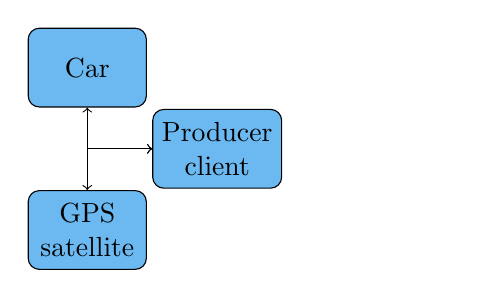
\begin{tikzpicture}[auto, node distance=1.5cm,
                stage/.style={rectangle, rounded corners, minimum width=1.5cm, minimum height=1cm,text centered, fill=diagramLight, draw, align=center},
                sharp/.style={rectangle, minimum width=9.0cm, minimum height=1cm,text centered, fill=diagramLight, draw, align=center},
                server/.style={rectangle, rounded corners, minimum width=1.5cm, minimum height=1cm,text centered, fill=diagramLight, rectangle split, rectangle split parts=2, draw},
                flow/.style={draw, ->},
                reverse_flow/.style={draw, <-},
                double_flow/.style={draw, <->},
                create/.style={draw, ->},
                use/.style={draw, dotted, ->}
            ]

            \node (backend) at (0,0) [draw=none] {};

            \node (web2) [draw=none, left=0.3cm of backend] {};

            \node (dataprov) [stage, left=0.3cm of web2] {Producer \\ client};
            \node (ghost1) [draw=none, left=0.7cm of dataprov] {};
            \node (car) [stage, above=0.4cm of ghost1] {Car};
            \node (sat) [stage, below=0.4cm of ghost1] {GPS \\ satellite};

            \node (web1) [draw=none, right=0.3cm of backend] {};

            \node (front) [draw=none, right=0.3cm of web1] {};

            \draw [double_flow] (dataprov) -| (sat);
            \draw [double_flow] (dataprov) -| (car);
        \end{tikzpicture}
    \end{figure}
    \note<1->[item]{\textbf{Producer client}, collection of data, different data sources, car, gps, camera etc.}
    \note<1->[item]{\textbf{Car}, OBD, other sources of data}
    \note<1->[item]{\textbf{GPS}, position data, time, speed}
\end{frame}

\begin{frame}{System overview}
    \framesubtitle{Overview of the system}
    \begin{figure}
        \pgfdeclarelayer{background}
        \pgfsetlayers{background,main}
        \tikzstyle{bgbox}=[fill=green!20, rounded corners, draw=GoogleGreen, dashed]
        \center
        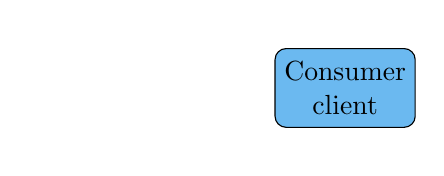
\begin{tikzpicture}[auto, node distance=1.5cm,
                stage/.style={rectangle, rounded corners, minimum width=1.5cm, minimum height=1cm,text centered, fill=diagramLight, draw, align=center},
                sharp/.style={rectangle, minimum width=9.0cm, minimum height=1cm,text centered, fill=diagramLight, draw, align=center},
                server/.style={rectangle, rounded corners, minimum width=1.5cm, minimum height=1cm,text centered, fill=diagramLight, rectangle split, rectangle split parts=2, draw},
                flow/.style={draw, ->},
                reverse_flow/.style={draw, <-},
                double_flow/.style={draw, <->},
                create/.style={draw, ->},
                use/.style={draw, dotted, ->}
            ]

            \node (backend) at (0,0) [draw=none] {};

            \node (web2) [draw=none, left=0.3cm of backend] {};

            \node (dataprov) [draw=none, left=0.3cm of web2] {};
            \node (ghost1) [draw=none, left=0.7cm of dataprov] {};
            \node (car) [draw=none, above=0.4cm of ghost1] {};
            \node (sat) [draw=none, below=0.4cm of ghost1] {};

            \node (web1) [draw=none, right=0.3cm of backend] {};

            \node (front) [stage, right=0.3cm of web1] {Consumer \\ client};
        \end{tikzpicture}
    \end{figure}
    \note<1->[item]{\textbf{Consumer client}, different types, BI system, DW system, GUI of back--end, what needs the data}
\end{frame}

\begin{frame}{System overview}
    \framesubtitle{Overview of the system}
    \begin{figure}
        \pgfdeclarelayer{background}
        \pgfsetlayers{background,main}
        \tikzstyle{bgbox}=[fill=green!20, rounded corners, draw=GoogleGreen, dashed]
        \center
        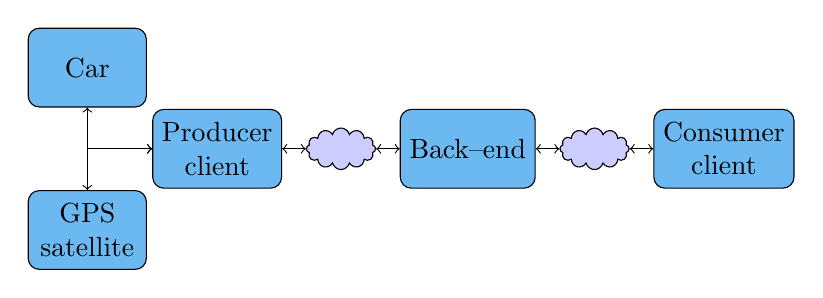
\begin{tikzpicture}[auto, node distance=1.5cm,
                stage/.style={rectangle, rounded corners, minimum width=1.5cm, minimum height=1cm,text centered, fill=diagramLight, draw, align=center},
                sharp/.style={rectangle, minimum width=9.0cm, minimum height=1cm,text centered, fill=diagramLight, draw, align=center},
                server/.style={rectangle, rounded corners, minimum width=1.5cm, minimum height=1cm,text centered, fill=diagramLight, rectangle split, rectangle split parts=2, draw},
                flow/.style={draw, ->},
                reverse_flow/.style={draw, <-},
                double_flow/.style={draw, <->},
                create/.style={draw, ->},
                use/.style={draw, dotted, ->}
            ]
            %, line width=0.5mm, draw=black
            \node (backend) at (0,0) [stage] {Back--end};

            \node (web2) [draw, cloud, cloud puffs=12, cloud ignores aspect, minimum width=2.5em, minimum height=1.5em,fill=blue!20, left=0.3cm of backend] {};

            \node (dataprov) [stage, left=0.3cm of web2] {Producer \\ client};
            \node (ghost1) [draw=none, left=0.7cm of dataprov] {};
            \node (car) [stage, above=0.4cm of ghost1] {Car};
            \node (sat) [stage, below=0.4cm of ghost1] {GPS \\ satellite};

            \node (web1) [draw, cloud, cloud puffs=12, cloud ignores aspect, minimum width=2.5em, minimum height=1.5em,fill=blue!20, right=0.3cm of backend] {};

            \node (front) [stage, right=0.3cm of web1] {Consumer \\ client};

            \draw [double_flow] (backend) -- (web2);
            \draw [double_flow] (web2) -- (dataprov);

            \draw [double_flow] (dataprov) -| (sat);
            \draw [double_flow] (dataprov) -| (car);

            \draw [double_flow] (backend) -- (web1);
            \draw [double_flow] (web1) -- (front);
        \end{tikzpicture}
    \end{figure}
    \note<1->[item]{\textbf{Back--end}, combine producer and consumer, our focus, REST API, db}
    \note<1->[item]{normalise data at producer client, back--end don't about data source}
    \note<1->[item]{neutral data, different devices: tablets, web, etc.}
    \note<1->[item]{Troels talk more about the back--end.}
\end{frame}
\subimport{slides/restapi/}{content.tex}
\subimport{slides/problems/}{index.tex}
\subimport{slides/testing/}{index.tex}
\subimport{slides/ConsumerClient/}{index.tex}

% ====================================================

% Final slide
{\aauwavesbg
  \begin{frame}[plain,noframenumbering]
    \finalpage{\texttt{\textbf{return} PresentationStatus.Completed;}}
  \end{frame}}

\end{document}
